%%%%%%%%%%%%%%%%%%% EJERCICIO 3 %%%%%%
\textbf{Ejemplo 3 }\\
Se concede un préstamo de 2.000.000 COP, con un plazo de gracia muerto de 6 meses seguido de 4 cuotas trimestrales crecientes en un 10\%  y con un interés del 44\% nominal anual trimestre vencido. Elaborar la tabla de amortización.\\

%\newpage %USAR SOLO SI EL SOLUCIÓN QUEDA SOLO Y ES NECESARIO BAJARLO A LA SIGUIENTE PAGINA
\textbf{Solución.}\\
%La tabla ira centrada
\begin{center}
	\renewcommand{\arraystretch}{1.5}% Margenes de las celdas
	%Creación de la cuadricula de 3 columnas
	\begin{longtable}[H]{|c|c|c|}
		%Creamos una linea horizontal
		\hline
		%Definimos el color de la primera fila
		\rowcolor[HTML]{FFB183}
		%%%%% INICIO ASIGNACIÓN FECHA FOCAL %%%%%%%
		%%%%%%%%%% INICIO TITULO
		%Lo que se hace aquí es mezclar las 3 columnas en una sola
		\multicolumn{3}{|c|}{\cellcolor[HTML]{FFB183}\textbf{1. Asignación período focal}}  \\ \hline
		\multicolumn{3}{|c|}{$pf = \textit{0 ptv}$}   \\\hline
		%%%%%%%%%% FIN TITULO
		%%%%% INICIO DECLARACIÓN DE VARIABLES %%%%%%%
		%%%%%%%%%% INICIO TITULO
		%Lo que se hace aquí es mezclar las 3 columnas en una sola
		\multicolumn{3}{|c|}{\cellcolor[HTML]{FFB183}\textbf{2. Declaración de variables}}   \\ \hline
		%%%%%%%%%% FIN TITULO
		%%%%%%%%%% INICIO DE MATEMÁTICAS
		%Cada & hace referencia al paso de la siguiente columna
		\multicolumn{2}{|c|}{$\hspace{2 cm}VP= 2.000.000 \ COP \hspace{2 cm}$} & $i\equiv 11\% \textit{ ptv}$ \\
		\multicolumn{2}{|c|}{$\hspace{2 cm}g=10\% \hspace{2 cm}$} & $j=44\% \textit{ natv}$ \\
		\multicolumn{2}{|c|}{$\hspace{2 cm}n=4 \textit{ ptv} \hspace{2 cm}$} & $\hspace{2 cm}R = ? COP\hspace{2 cm}$ \\ \hline
		
		
		
		%%%%%%%%%% FIN DE MATEMÁTICAS
		%%%%% FIN DECLARACIÓN DE VARIABLES
		
		
		%%%%% INICIO FLUJO DE CAJA
		\rowcolor[HTML]{FFB183}
		\multicolumn{3}{|c|}{\cellcolor[HTML]{FFB183}\textbf{3. Diagrama de flujo de caja}} \\ \hline
		%Mezclamos 3 columnas y pondremos el dibujo
		%%%%%%%%%%%%% INSERCIÓN DE LA IMAGEN
		%Deberán descargar las imágenes respectivas del drive y pegarlas en la carpeta
		%n_capitulo/img/ejemplos/1/capitulo1ejemplo1.pdf  (el /1/ es el numero del ejemplo)
		\multicolumn{3}{|c|}{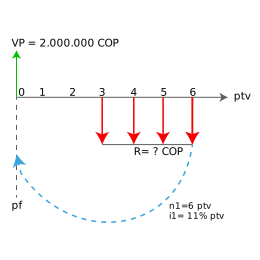
\includegraphics[trim=-78 -5 -78 -5]{7_Capitulo/img/ejemplos/3/Capitulo7Ejercicio3.pdf} }
		
		
		\\ \hline
		%%%%%%%%%%%%% FIN INSERCIÓN DE IMAGEN
		%%%%%FIN FLUJO DE CAJA
		
		
		
		%%%%% INICIO DECLARACIÓN FORMULAS
		%%%%%%%%%%% INICIO TITULO
		\rowcolor[HTML]{FFB183}
		\multicolumn{3}{|c|}{\cellcolor[HTML]{FFB183}\textbf{4. Declaración de fórmulas}}    \\ \hline
		%%%%%%%%%%% FIN TITULO
		%%%%%%%%%%% INICIO MATEMÁTICAS
		\multicolumn{3}{|c|}{$VP=R(\frac{R(1+g)^{n}(1+i)^{n}-1}{g-i}) \hspace{0.4 cm} \textit{Valor presente gradiente aritmetico}$} \\ \hline
		
		%%%%%%%%%% FIN MATEMÁTICAS
		%%%%%% INICIO DESARROLLO MATEMÁTICO
		\rowcolor[HTML]{FFB183}
		%%%%%%%%%%INICIO TITULO
		\multicolumn{3}{|c|}{\cellcolor[HTML]{FFB183}\textbf{5. Desarrollo matemático}}       \\ \hline
		%%%%%%%%%% FIN TITULO
		%%%%%%%%%% INICIO MATEMÁTICAS
		\multicolumn{3}{|c|}{$  2.000.000 \ COP = R(\frac{[(1+0.1)^{4}(1+0.11)^{-4}-1]}{0.1-0.11})(1+0.11)^{-2}\hspace{0.2 cm}\rightarrow \hspace{0.2 cm}R= 693.125,94 \ COP$} \\ \hline
		
		%%%%%%%%%% FIN MATEMÁTICAS
		%%%%%% FIN DESARROLLO MATEMÁTICO
		%%%%%% INICIO RESPUESTA
		\rowcolor[HTML]{FFB183}
		%%%%%%%%%%INICIO TITULO
		\multicolumn{3}{|c|}{\cellcolor[HTML]{FFB183}\textbf{6. Respuesta}}   \\ \hline
		%%%%%%%%%% FIN TITULO
		%%%%%%%%%% INICIO RESPUESTA MATEMÁTICA
		\multicolumn{3}{|c|}{$\mathbf{R= 693.125,94 \ COP}$}
		\begin{comment}
		\multicolumn{3}{|p{\textwidth}|}{
		$F_{4} = F_{5} = 21.609,84 \ COP $ .}
		\end{comment} 
		\\ \hline
		%%%%%%%%%% FIN MATEMÁTICAS
		%%%%%% FIN RESPUESTA
	\end{longtable}
	%Se crean dos lineas en blanco para que no quede el siguiente texto tan pegado
	%\newline \newline %USARLO SI CREES QUE ES NECESARIO
\end{center}
%%%%%%%%%%%%%%%%%%%%%%%%%%FIN EJERCICIO 3 %%%%%%%%%%%%%%%%%%%%%%%%%%%